\documentclass[../resumosRCOM.tex]{subfiles}
\usepackage[utf8]{inputenc}
\usepackage{graphicx}

\title{rcomTransport}
\author{p21silva98 }
\date{January 2019}

\begin{document}

\subsection{Services provided to the uppper layers}

\begin{figure}[h]
    \centering
    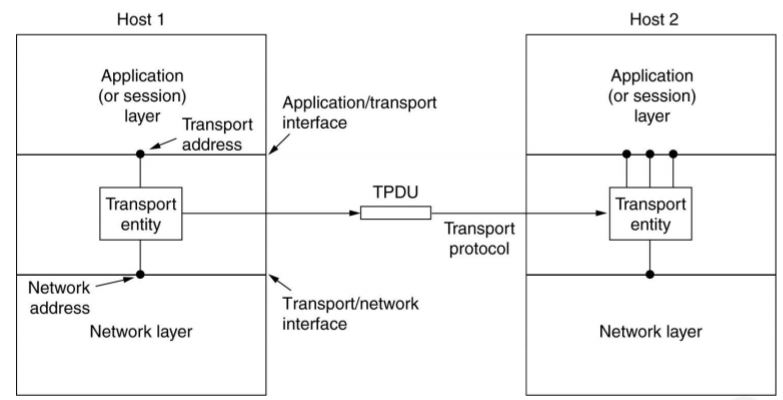
\includegraphics[width=7cm]{images/trans1.JPG}
\end{figure}

\subsection{Transport Service Primitives}
\begin{figure}[h]
    \centering
    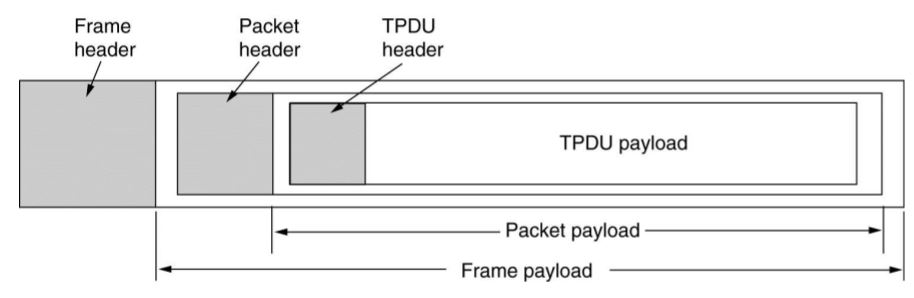
\includegraphics[width=11cm]{images/trans2.JPG}
\end{figure}

\subsection{UDP - User Datagram Protocol}
\textbf{Datagram oriented} \\
Unreliable because no error control mechanism\\ 
Connectionless\\
\textbf{Allows applications} \\
to interface directly to IP with minimal additional protocol overhead\\
\textbf{UDP header} \\
Port numbers identify sending and receiving processes \\
UDP length = length of packet in bytes \\
Checksum covers header and data; optional \\
\begin{figure}
    \centering
    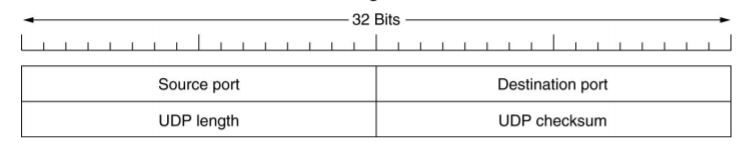
\includegraphics[width=11cm]{images/trans3.JPG}
\end{figure}

\subsection{TCP - Transmission Control Protocol}
\textbf{Flow Control}\\
Reliability\\
ARQ mechanism (error control with ACK)\\
Avoids receiver's congestion\\
\textbf{Congestion Control}\\
Avoids network's congestion\\
\textbf{Properties}\\
Connection oriented\\
Full-duplex\\
Byte stream\\
\begin{figure}[h]
    \centering
    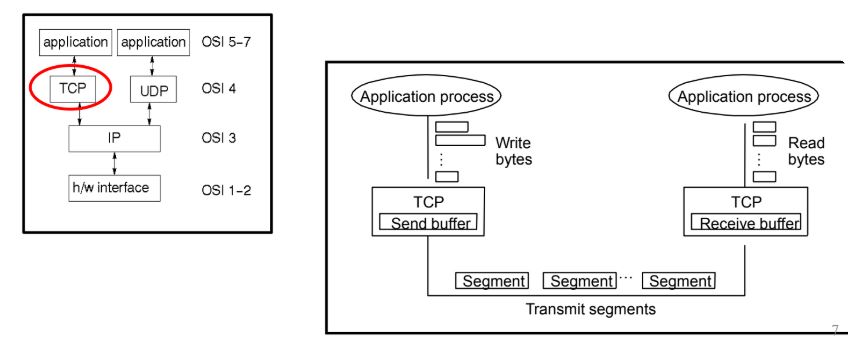
\includegraphics[width=11cm]{images/trans5.JPG}
\end{figure}

\subsection{Basic TCP Operation}
\textbf{-Sender}\\
Application data is broken in segments\\
TCP uses timer while waiting for an ACK of every segment sent\\
Un-ACKed segments are retransmitted\\
\textbf{-Receiver}\\
Errors detected using a checksum\\
Correctly received data is acknowledged\\
Segments reassembled in proper order\\
Duplicated segments discarded\\
\textbf{-Window based flow control}

\subsection{The TCP Segment Header}
\begin{figure}[h]
    \centering
    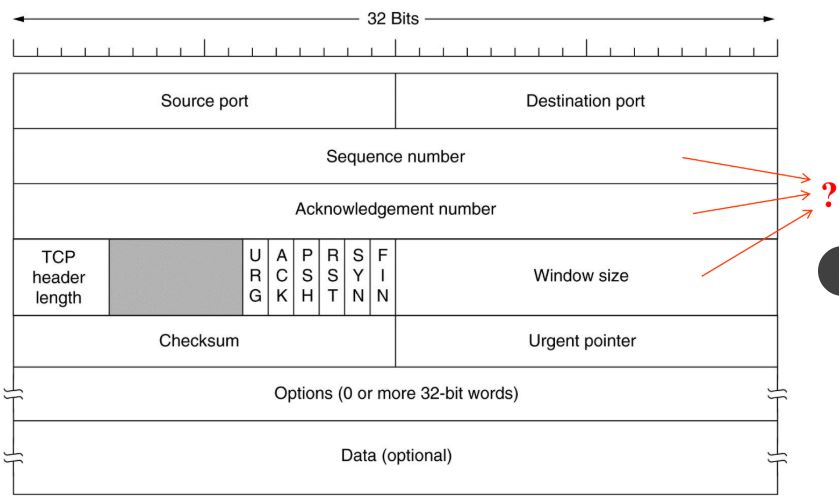
\includegraphics[width=11cm]{images/trans6.JPG}
\end{figure}

\subsection{TCP Header}
\begin{itemize}
    \item Ports number are the same as for UDP
    \item 32 bit SeqNumber uniquely identifies the application data contained in the TCP segment
    \begin{itemize}
        \item SeqNumber is in bytes
        \item It identifies the first byte of data
    \end{itemize}
    \item 32 bit AckNumber is used for piggybacking ACKs
    \begin{itemize}
        \item AckNumber indicates the next byte the receiver is expecting
        \item Implicit ACK for all the bytes up to that point
    \end{itemize}
    \item Window size
    \begin{itemize}
        \item Used for control (ARQ) and congestion control
        \begin{itemize}
            \item Sender cannot have more than a window of bytes in the network
        \end{itemize}
        \item Specified in bytes
        \begin{itemize}
            \item Window scaling used to increase the window size in high speed networks
        \end{itemize}
    \end{itemize}
    \item Checksum covers the header and data
\end{itemize}

\subsection{Sequence Numbers in TCP}
\begin{itemize}
    \item TCP regards data as byte-stream (each byte is numbered sequentially)
    \item TCP breaks byte stream into segments (size limited by the Maximum Segment Size - MSS)
    \item Each packet has a sequence numbe (sequence number of 1st byte of data transported by the segment)
    \item TCP connection is duplex (data in each direction has different sequence numbers)
\end{itemize}

\subsection{Connection Establishment}
\begin{figure}[h]
    \centering
    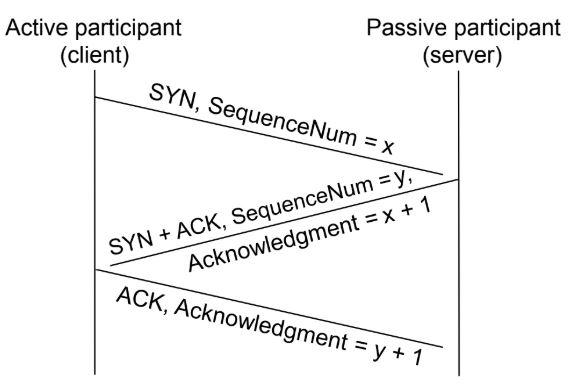
\includegraphics[width=11cm]{images/trans7.JPG}
\end{figure}

\subsection{TCP connection management}
\begin{figure}[h]
    \centering
    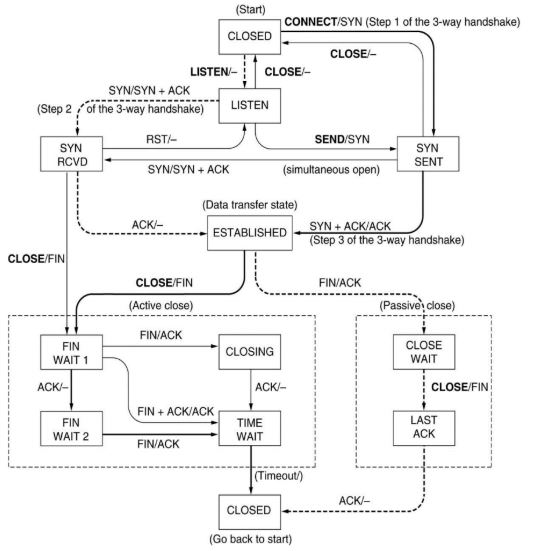
\includegraphics[width=11cm]{images/trans8.JPG}
\end{figure}

\subsection{Retransmissions in TCP - A variation of Go-Back-N}
\begin{itemize}
    \item Sliding Window
    \begin{itemize}
        \item Ack contains a single sequence number
        \item Acknowledges all bytes with a lower sequence number
        \item Duplicate ACKs sent when out-of-order packet received
    \end{itemize}
    \item  Sender retransmits a single packet at a time
    \begin{itemize}
        \item optimistic assumption - only one packet is lost
    \end{itemize}
    \item Error control based on byte sequences, not packets
\end{itemize}

\subsection{Sliding Window}
\begin{itemize}
    \item Sender
    \begin{itemize}
        \item LastByteAcked less or equal than LastByteSent
        \item LastByteSent less or equal than LastByteWritten
        \item Buffers bytes between LastByteAcked and LastByteWritten
    \end{itemize}
    \item Receiver
    \begin{itemize}
        \item LastByteRead less than NextByteExpected
        \item LastByteExpected less or equal than LastByteRcvd + 1
        \item Buffers bytes between LastByteRead and LastByteRcvd
    \end{itemize}
\end{itemize}
\begin{figure}[h]
    \centering
    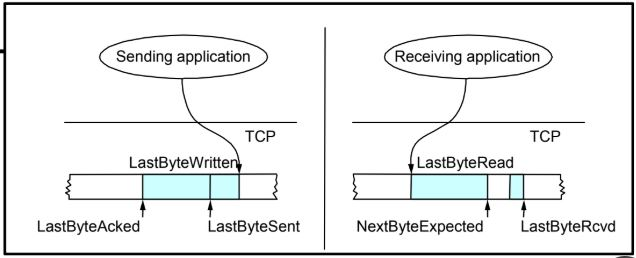
\includegraphics[width=11cm]{images/trans9.JPG}
\end{figure}

\subsection{Flow Control}
\begin{itemize}
    \item Buffer length
    \begin{itemize}
        \item Sender - MaxSendBuffer
        \item Receiver - MaxRcvBuffer
    \end{itemize}
    \item Receiver
    \begin{itemize}
        \item LastByteRcvd - LastByteRead less or equal than MaxRcvBuffer
        \item AdvertisdeWindow equals MaxRcvBuffer - (LastByteRcvd - LastByteRead) 
    \end{itemize}
    \item Sender
    \begin{itemize}
        \item LastByteWritten - LastByteAcked less or = MaxSendBuffer
        \item LastByteSent - LastByteAcked less or = AdvertisedWindow
        \item EffectiveWindow = AdvertisedWindow - (LastByteSent - LastByteAcked)
    \end{itemize}
    \item Sending application blocks if it needs to write y bytes and (LastByteWritten - LastByeAcked) + y greater than MaxSenderBuffer
    \item ACK sent when a segment is received
\end{itemize}

\subsection{Adaptive Retransmission (Original Algorithm)}
\begin{itemize}
    \item RTT - Round trip time
    \item sampleRTT measured for each segment/ACK pair
    \item Average RTT (RTT = a * RTT + (1-a) * sampleRTT) a in [0.8,0.9]
    \item Timeout = 2 * RTT
\end{itemize}

\subsection{Karn/Partride Algorithm}
\begin{itemize}
    \item sampleRTT not measured in retransmission
    \item Timeout doubled for each retransmission
\end{itemize}
\begin{figure}[h]
    \centering
    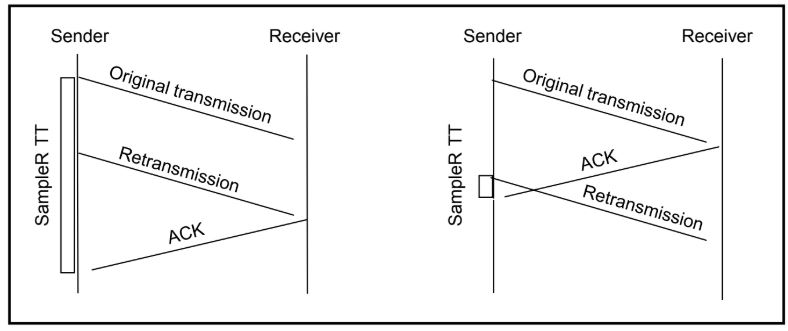
\includegraphics[width=11cm]{images/trans10.JPG}
\end{figure}

\subsection{Selective ACK}
\begin{itemize}
    \item Option for selective ACKs (SACK) also widely deployed
    \item Selective acknowledgement (SACK)
    \begin{itemize}
        \item adds a bitmask of packets received
        \item implemented as a TCP option
    \end{itemize}
    \item When to retransmit?
    \begin{itemize}
        \item packets may experience different delays
        \item still need to deal with reordering
        \item wait for out of order by 3 packets
    \end{itemize}
\end{itemize}

\subsection{TCP- Congestion Control}
Each source determines its capicity.\\
Its based on criteria enablind \textbf{flow fairness} and \textbf{efficiency}.\\
Received ACKs regulate packet transmission, they are used as the source clock.\\

\subsection{Additive Increase/Multiplicative Decrease}
Changes in channel capacity leads to adjustment of transmission rate.\\
New variable per connection (CongestionWindow)\\
Limits the amout of traffic in transit :\\
MaxWin = MIN(CongestionWindow, AdvertisedWindow)\\
EffWin = MaxWin - (LastByteSent - LastByteAcked)\\

\begin{figure}[h]
    \centering
    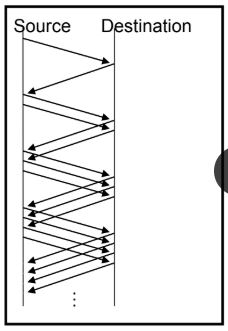
\includegraphics[width=7cm]{images/trans11.JPG}
\end{figure}

\textbf{Objective}\\
If network congestion \textbf{decreases} then CongestionWindow \textbf{increases}.\\
If network congestion \textbf{increases} then CongestionWindow \textbf{decreases}.\\
\textbf{Bitrate(byte/s) = CongestionWindow/RTT}\\

\textbf{How to know if/when network is in congestion?} Timeout!\\
Timeout occurence leads to loss of packet. Packet loss leads to buffer in router is full which leads to congestion. //

\subsubsection{Algorithm}
\begin{itemize}
    \item increases CongestionWindow by 1 segment. For each RTT - additive increase
    \item divide CongestionWindow by 2. When there is a packet loss - multiplicative decrease.
\end{itemize}

\subsubsection{In practice}
\begin{itemize}
    \item Increases by ACK received
    \item Increment = MSS * (MSS / CongestionWindow)
    \item CongestionWindow += Increment
    \item MSS = Maximum Segment Size
\end{itemize}

\subsubsection{Objective}
Determine the available capacity

\subsubsection{Behaviour}
Start by CongestionWindow = 1 segment. \\
Double CongestionWindow by each RTT.\\

\subsection{Fast Retransmission, Fast Recovery}
\textbf{Problem}
If TCP timeout is large then long inactivity period
\begin{figure}[h]
    \centering
    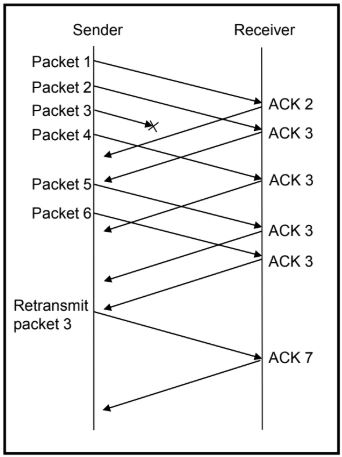
\includegraphics[width=7cm]{images/trans12.JPG}
\end{figure}

\textbf{Solution}
Fast retransmission - after 3 repeated ACK's

\subsection{TCP - Slow start}
\begin{figure}[h]
    \centering
    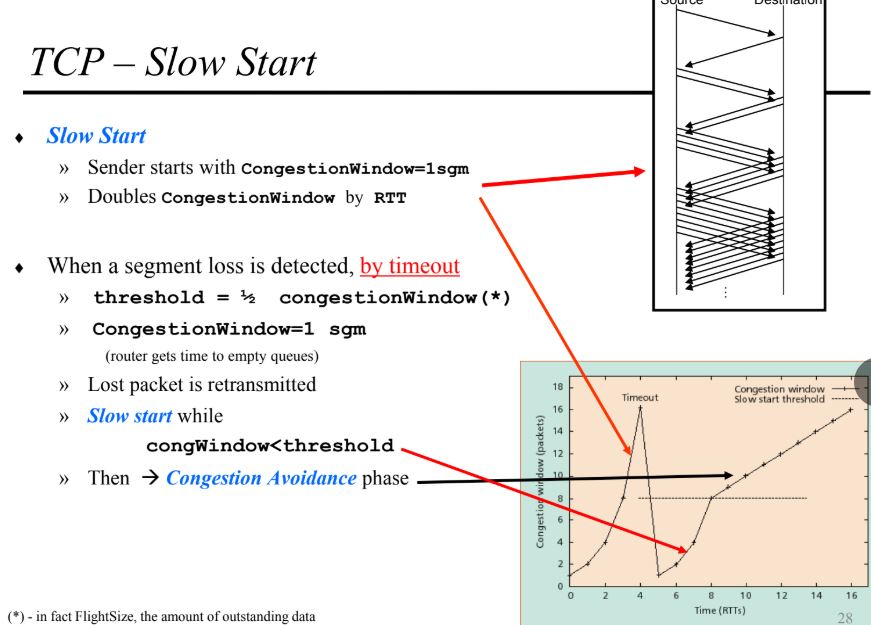
\includegraphics[width=11cm]{images/trans13.JPG}
\end{figure}

\subsection{Congestion Avoidance}
\begin{itemize}
    \item Congestion Avoidance (additive increase)
    \begin{itemize}
        \item increments congestionWindow by 1sgm, per RTT
    \end{itemize}
    \item Detection of segment loss, by reception of 3 duplicated ACKs
    \begin{itemize}
        \item Assumes packet is lost (because following segments have arrived)
        \item Retransmits lost packet
        \item CongestionWindow = CongestionWindow/2
        \item Congestion Avoidance Phase
    \end{itemize}
\end{itemize}
\begin{figure}[h]
    \centering
    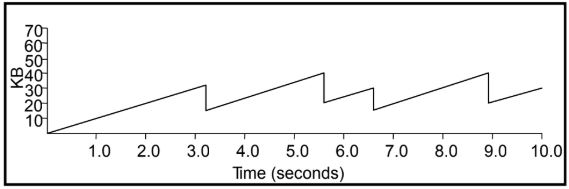
\includegraphics[width=11cm]{images/trans14.JPG}
\end{figure}

\subsection{Desirable Bandwidth Allocation}
\begin{figure}[h]
    \centering
    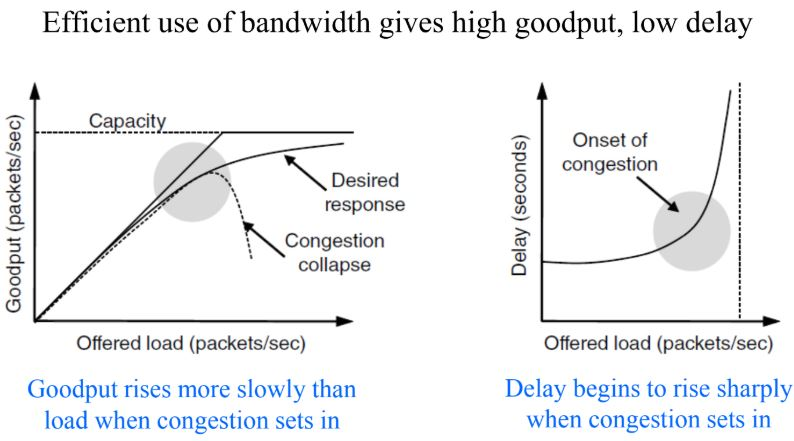
\includegraphics[width=11cm]{images/trans15.JPG}
\end{figure}

\subsection{Max-min fairness}
\begin{figure}[h]
    \centering
    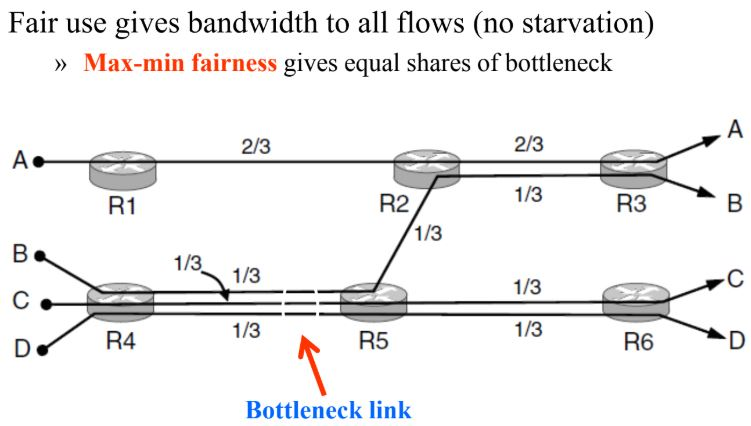
\includegraphics[width=11cm]{images/trans16.JPG}
\end{figure}

\subsection{Bitrates along the time}
\begin{figure}[h]
    \centering
    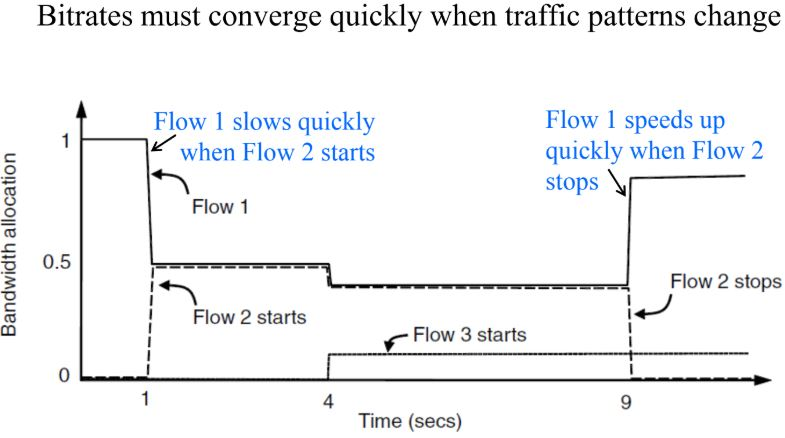
\includegraphics[width=11cm]{images/trans17.JPG}
\end{figure}


\end{document}
